\documentclass[12pt,compress,usenames,dvipsnames,aspectratio=169]{beamer}
\usetheme[sidebarleft]{Singapore}
\useoutertheme{shadow}
%\usetheme{CambridgeUS}
\definecolor{mygreen}{RGB}{150, 255, 210}%186}
\definecolor{leftblue}{RGB}{230,255,255}
\definecolor{rightblue}{RGB}{111,195,223}
\definecolor{lefttron}{RGB}{19,44,65}
\definecolor{myblack}{RGB}{27,27,27}
\definecolor{mypurple}{RGB}{205,87,255}

\usecolortheme{owl}

% \setbeamercolor{section in head/foot}{fg = white,bg=black}
\setbeamercolor{title}{fg=mygreen,bg=black}
\setbeamercolor{titlelike}{fg=yellow,bg=black}
\setbeamercolor{item}{fg=mygreen}
\setbeamercolor{block title}{fg=white,bg=myblack!200}
\setbeamercolor{block body}{bg=normal text.bg!80}
\setbeamertemplate{blocks}[rounded][shadow=true]
\setbeamertemplate{headline}{}
\setbeamertemplate{footline}[frame number]
\setbeamercolor{normal text}{fg=white,bg=myblack}%!89.9}

%Gradient
\setbeamercolor{frametitle}{fg=orange,bg=black}
\setbeamercolor{frametitle right}{fg=white,bg=gray}

\usepackage[spanish]{babel}
\usepackage[utf8]{inputenc}
\usepackage{amsmath}
\usepackage{amsfonts}
\usepackage{amssymb}
\usepackage{graphicx}
\usepackage{shadowtext}
\usepackage{multicol}
\usepackage[makeroom]{cancel}

%\graphicspath{{./figures/},
%}

%\AtBeginSection{\frame{\sectionpage}}

%\usepackage{natbib}
\usepackage{float}
\usepackage{subcaption}
%\usepackage{xcolor}
%\usepackage{natbib}
\usepackage{bibentry}
\usepackage{animate}
\usepackage{varwidth}
%\usepackage{appendixnumberbeamer}

\usepackage{tikz}
\usetikzlibrary{shapes,arrows}

\title{\textbf{Muestreo estratificado}}
\author{Aurora Rios Medina \\
Jose Manuel Gonzalez Alcantara \\
Juan Carlos Escobar Teja \\
Osmar Dominique Santana Reyes}

\date{\today}

\usefonttheme{professionalfonts}

%\usepackage{mydefs}

\setbeamercovered{transparent} 
\setbeamertemplate{navigation symbols}{} 
%\titlegraphic{
%\begin{center}
%\vspace*{-30pt}
%\includegraphics[height=0.15\tH]{figures/uni_logo.png}
%
%\vspace*{10pt}
%\includegraphics[height=0.03\tH]{figures/mail_logo.png}\hspace*{2pt}
%{\scriptsize \href{mailto:abarik@jhu.edu}{email@example.com}}\hspace*{20pt}
%\includegraphics[height=0.03\tH]{figures/twit.png}\hspace*{2pt}
%{\scriptsize \href{https://twitter.com/MHDwizard}{@TwitterHandle}}
%\end{center}
%}
%\institute[JHU]{Planetary Interiors}



\begin{document}

\frame{\titlepage}

\setbeamercovered{invisible}

\begin{frame}{Índice}
	\tableofcontents
\end{frame}

%----------------------------------------------------------------------------------------------------------------------

\section{4.1. ¿Qué es el muestreo estratificado?}
\begin{frame}{4.1. ¿Qué es el muestreo estratificado?}
    Muchas veces se cuenta con información extra acerca de una población, que puede ayudar a obtener una muestra más representativa. Por ejemplo, \vspace{0.5mm}

    \begin{minipage}[h]{0.4\linewidth}
        \begin{itemize}
            \item Al realizar una muestra sobre una población dada, para saber sobre el consumo de alimentos en la población. 
            
            %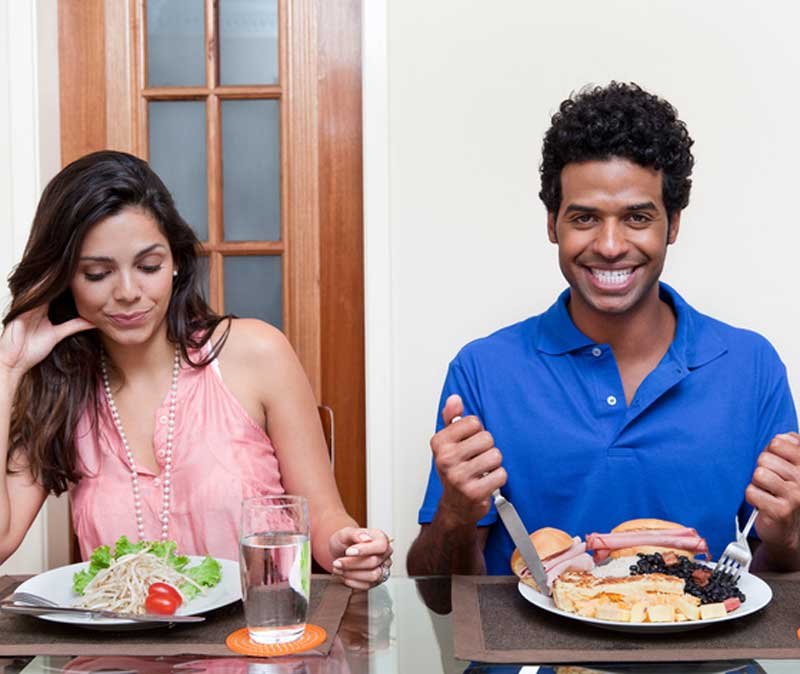
\includegraphics[width = 0.9\linewidth]{MujervsHombre.jpg}
        \end{itemize}
    \end{minipage} \hspace{0.05\linewidth}
    \begin{minipage}[h]{0.45\linewidth}
        \begin{itemize}
            \item Los residentes rurales acuden más a una tienda que los residentes urbanos.
            
            %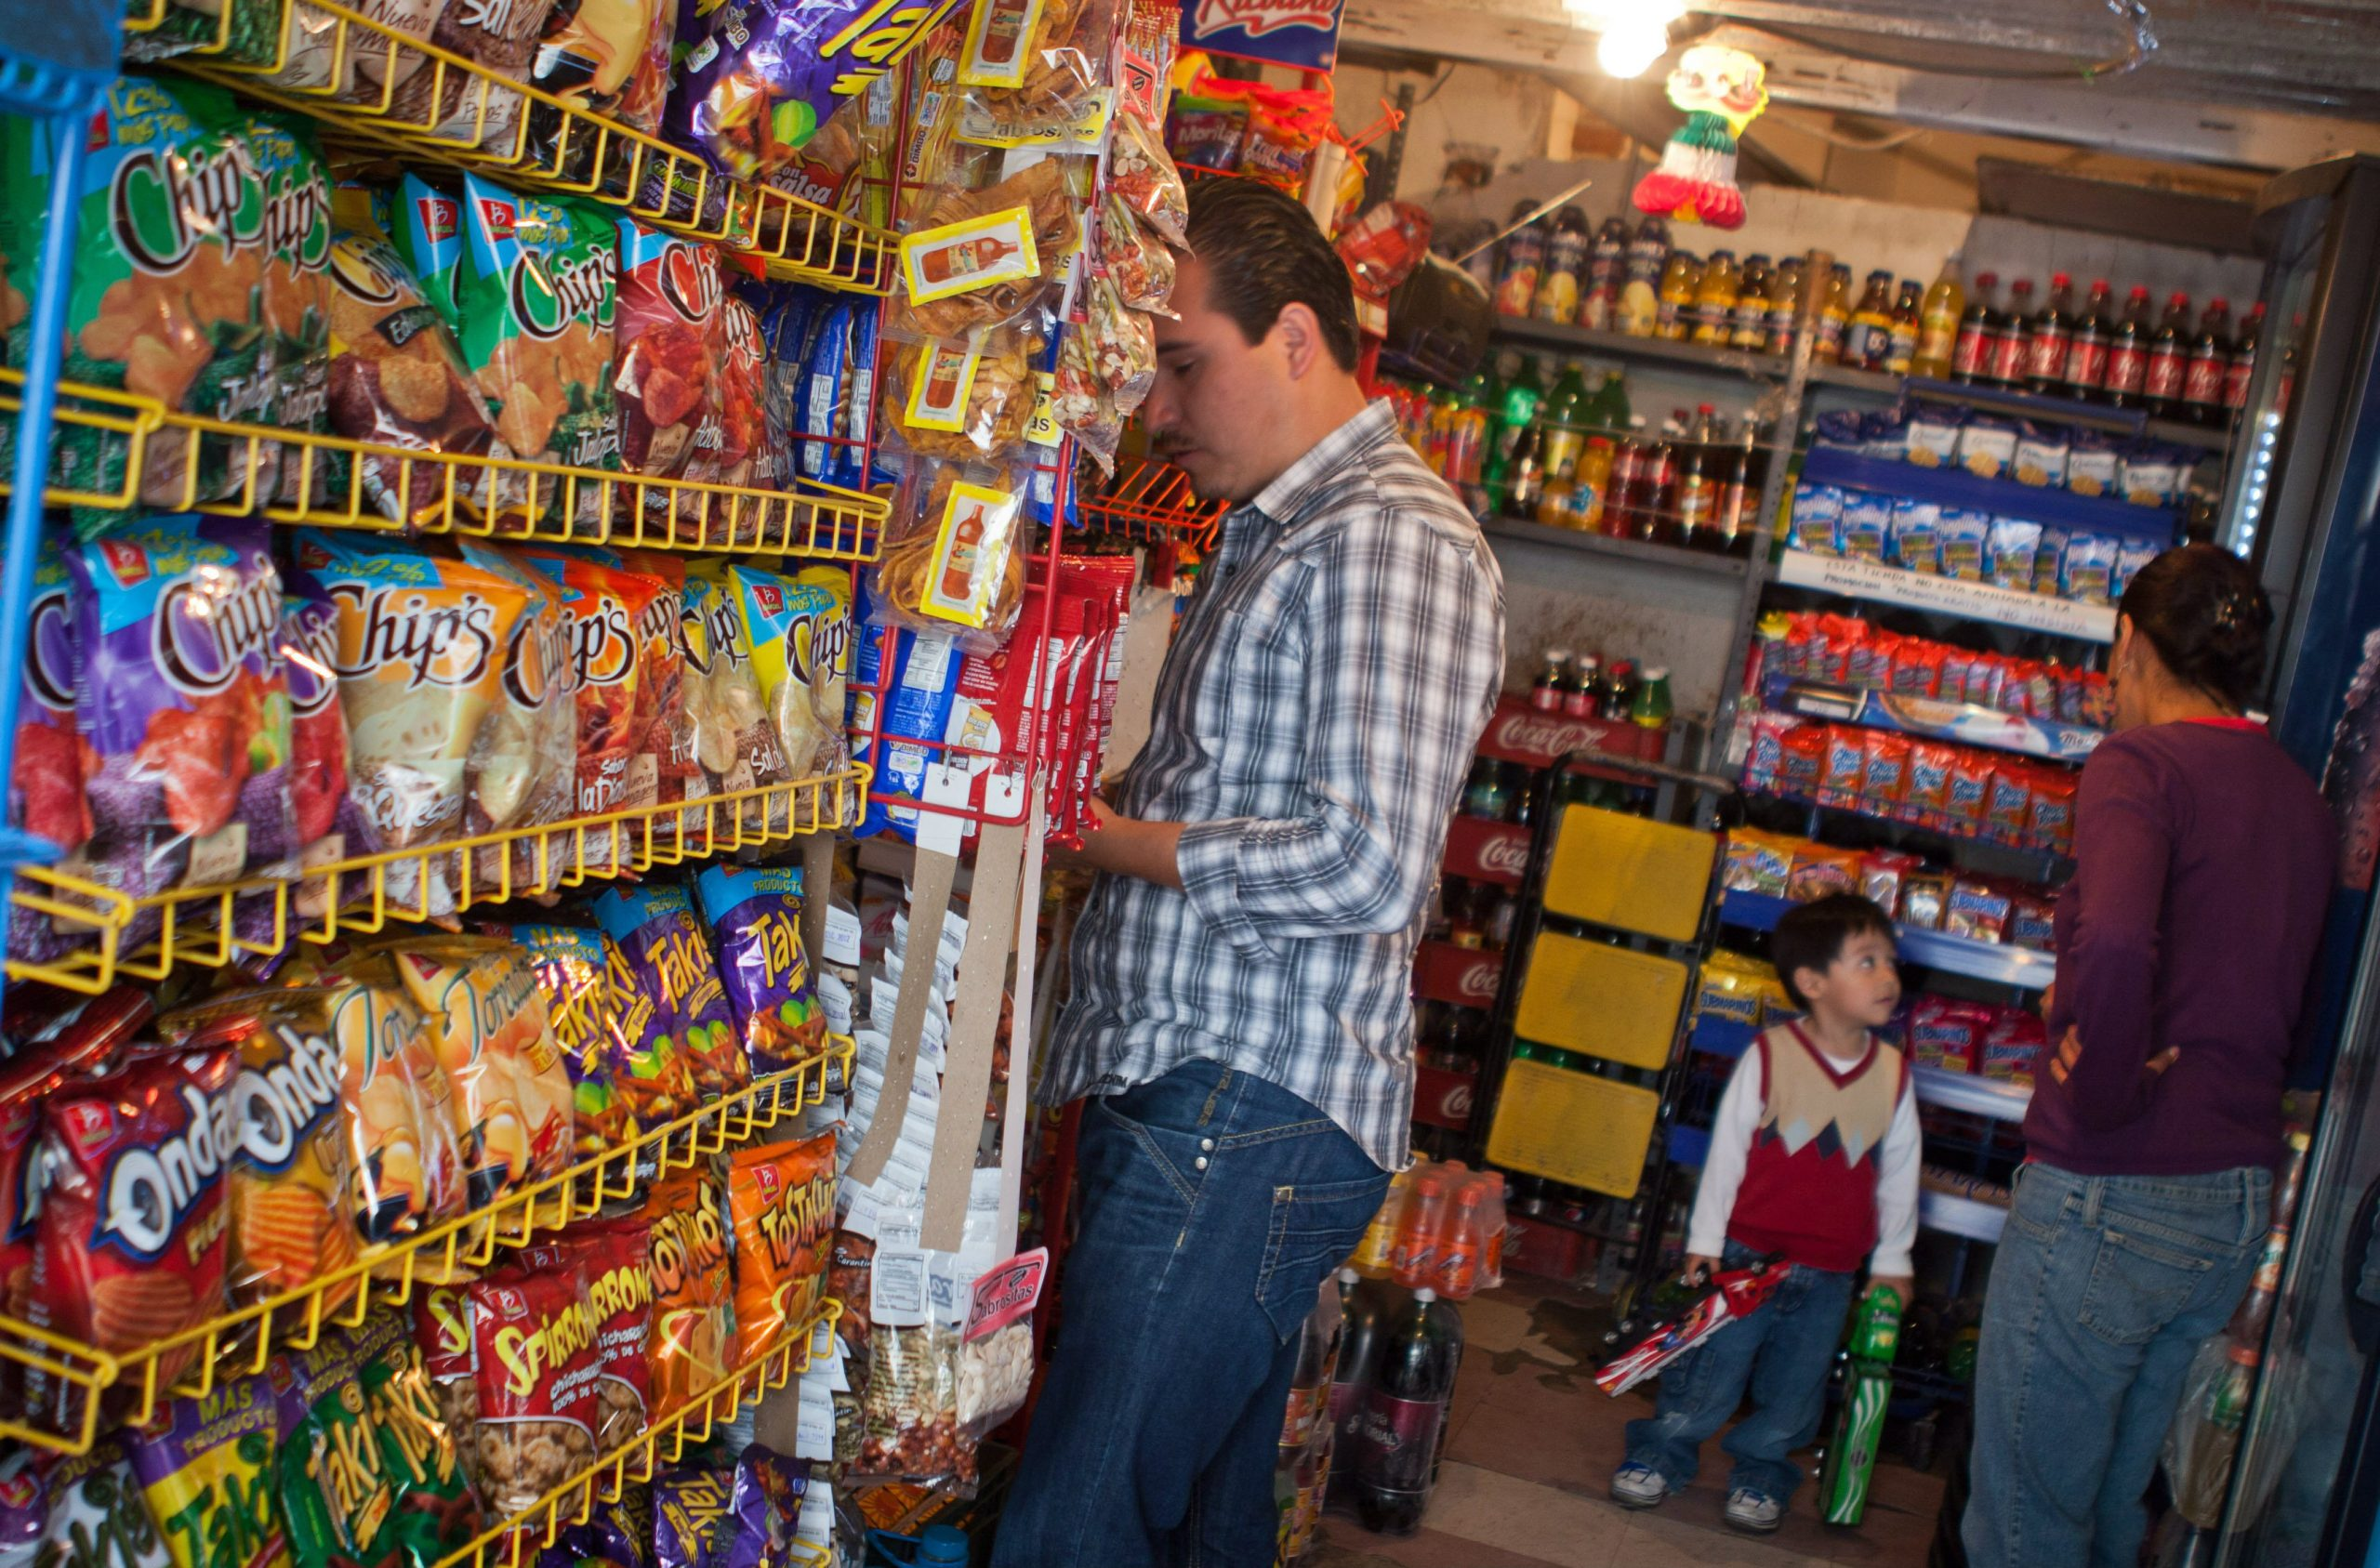
\includegraphics[width = 0.9\linewidth]{tienda.jpg}
        \end{itemize}
    \end{minipage}
\end{frame}

%----------------------------------------------------------------------------------------------------------------------

\begin{frame}
    Sea $ \Omega $ una población finita de $ N $ elementos y $ \left\lbrace \Omega_1, \Omega_2, \ldots, \Omega_m \right\rbrace $ una partición de $ \Omega $. A cada $ \Omega_i $, con $ i = 1, \ldots, m $ se le llama \textbf{estrato de la población}. 

    Para cada $ i = 1, \ldots, m $, sean $ N_i = \left| \Omega_i \right| $ y $ n_i $ el tamaño de una muestra obtenida de $ \Omega_i $. Las muestras obtenidas de cada estrato se juntan para formar una muestra de la población total, $ \Omega $.

    \textbf{Observaciones:}

    \begin{itemize}
        \item $ \sum_{i=1}^{m} N_i = N $
        \item Los métodos de muestreo utilizados en cada estrato no tienen que ser iguales y pueden ser independientes o no.
        \item Cuando las muestras de cada estrato sean aleatorias, al procedimiento completo se le llamará \textbf{Muestreo aleatorio estratificado}.
    \end{itemize}
\end{frame}

%-----------------------------------------------------------------------------------------------------------------------

\begin{frame}
    \frametitle{Razones para usar el muestreo estratificado}

    

\end{frame}

\end{document}